% !TEX program = xelatex
\documentclass[10pt,letterpaper,twocolumn]{article}

% === GEOMETRY ===
\usepackage[top=0.75in, bottom=0.75in, left=0.75in, right=0.75in, footskip=12pt]{geometry}

% === FONTS ===
\usepackage{fontspec}
\usepackage{unicode-math}
\setmainfont{Latin Modern Roman}[
  Extension=.otf,
  UprightFont=lmroman10-regular,
  BoldFont=lmroman10-bold,
  ItalicFont=lmroman10-italic,
  BoldItalicFont=lmroman10-bolditalic,
]
\setsansfont{Latin Modern Sans}[
  Extension=.otf,
  UprightFont=lmsans10-regular,
  BoldFont=lmsans10-bold,
  ItalicFont=lmsans10-oblique,
  BoldItalicFont=lmsans10-boldoblique,
]
\setmonofont{Latin Modern Mono}[
  Extension=.otf,
  UprightFont=lmmono10-regular,
  ItalicFont=lmmono10-italic,
  Scale=0.85,
]
% YWFT Processing is used in one place: the title.
\newfontfamily\acbold{ywft-processing-bold}[
  Path=../../system/public/type/webfonts/,
  Extension=.ttf
]

% === PACKAGES ===
\usepackage{xcolor}
\usepackage{colortbl}
\usepackage{titlesec}
\usepackage{enumitem}
\usepackage{tabularx}
\usepackage{fancyhdr}
\usepackage{hyperref}
\usepackage{xurl}
\usepackage{graphicx}
\graphicspath{{./}{figures/}}
\usepackage{ragged2e}
\usepackage{microtype}
\usepackage[font=footnotesize]{caption}
\usepackage{natbib}
\usepackage{balance}
\usepackage{tikz}
\usetikzlibrary{calc, positioning}

% === COLORS (AC palette) ===
\definecolor{acpink}{RGB}{180,72,135}
\definecolor{acpurple}{RGB}{120,80,180}
\definecolor{acdark}{RGB}{64,56,74}
\definecolor{acgray}{RGB}{119,119,119}
\definecolor{acgold}{RGB}{176,132,24}
\definecolor{tezblue}{RGB}{44,125,247}

% House table and source bundle live one directory up.
\makeatletter\def\input@path{{../}}\makeatother
\usepackage{ac-paper-table}
\usepackage{ac-source-bundle}
\newcolumntype{Y}{>{\raggedright\arraybackslash}X}
% Table colour carries meaning: teal for what held or shipped, pink for what
% was retracted or is missing, gold for what is partial or pending.
\definecolor{acheld}{RGB}{214,238,228}
\definecolor{acgone}{RGB}{251,223,233}
\definecolor{acpart}{RGB}{250,238,204}
\newcommand{\held}{\cellcolor{acheld}}
\newcommand{\gone}{\cellcolor{acgone}}
\newcommand{\partly}{\cellcolor{acpart}}
\newcolumntype{Q}[1]{>{\raggedright\arraybackslash}p{#1}}
% Pastel column coding: each column carries one tint.
\newcolumntype{T}[1]{>{\columncolor{#1}\raggedright\arraybackslash}X}
\newcolumntype{U}[2]{>{\columncolor{#1}\raggedright\arraybackslash}p{#2}}
\newcolumntype{V}[1]{>{\columncolor{#1}}l}

% === HYPERREF ===
\hypersetup{
  colorlinks=true,
  linkcolor=acpurple,
  urlcolor=acpurple,
  citecolor=acpurple,
  pdfauthor={@jeffrey},
  pdftitle={PLOrk'ing the Planet: A Laptop Orchestra That Boots from a USB Stick},
}

% === SECTION FORMATTING ===
\titleformat{\section}
  {\normalfont\bfseries\normalsize\raggedright\uppercase}
  {\thesection.}
  {0.5em}
  {}
\titlespacing{\section}{0pt}{1.2em}{0.3em}

\titleformat{\subsection}
  {\normalfont\bfseries\small}
  {\thesubsection}
  {0.5em}
  {}
\titlespacing{\subsection}{0pt}{0.8em}{0.2em}

% === HEADER/FOOTER ===
\pagestyle{fancy}
\fancyhf{}
\renewcommand{\headrulewidth}{0pt}
\fancyfoot[C]{\footnotesize\thepage}

% === CUSTOM COMMANDS ===
\newcommand{\acdot}{{\color{acpink}.}}
\newcommand{\ac}{Aesthetic{\acdot}Computer}
\newcommand{\acos}{AC Native OS}
\newcommand{\np}{\href{https://notepat.com}{\texttt{notepat}}}
% A handle is a person's address on the network: set in the house handle
% colour and linked to their page.
\definecolor{achandle}{RGB}{0,116,196}
\DeclareRobustCommand{\handle}[1]{\href{https://prompt.ac/@#1}{\textbf{\color{achandle}@#1}}}
\newcommand{\commit}[1]{\href{https://github.com/whistlegraph/aesthetic-computer/commit/#1}{\texttt{#1}}}
\newcommand{\key}[1]{\texttt{#1}}
% The tez mark is a vector drawing in figures/tez.pdf, so the paper builds
% on machines without a font that carries the glyph.

% Version stamp (hash + revision), regenerated by papers/cli.mjs on every
% build; the fallback keeps a manual xelatex run compiling.
\InputIfFileExists{version}{}{%
  \providecommand{\paperhash}{dev}\providecommand{\paperrev}{?}}
% Tezos edition: edition.tex names the one revision that was minted. The
% stamp at the end of the paper prints only while \paperrev matches it, so
% later revisions drop the mark without any edit here.
\InputIfFileExists{edition}{}{\providecommand{\editionrev}{none}}

% === LIST SETTINGS ===
\setlist[itemize]{nosep, leftmargin=1.2em, itemsep=0.1em}
\setlist[enumerate]{nosep, leftmargin=1.2em}

\setlength{\columnsep}{1.8em}
\setlength{\parindent}{1em}
\setlength{\parskip}{0.3em}

\raggedbottom
\setlength{\bibsep}{0.25em}
\tolerance=800
\emergencystretch=1em
\hyphenpenalty=50

\begin{document}

% ============ TITLE BLOCK ============

\twocolumn[{%
\begin{center}
{\acbold\fontsize{27pt}{31pt}\selectfont\color{acdark} PLOrk'ing the Planet}\par
\vspace{0.4em}
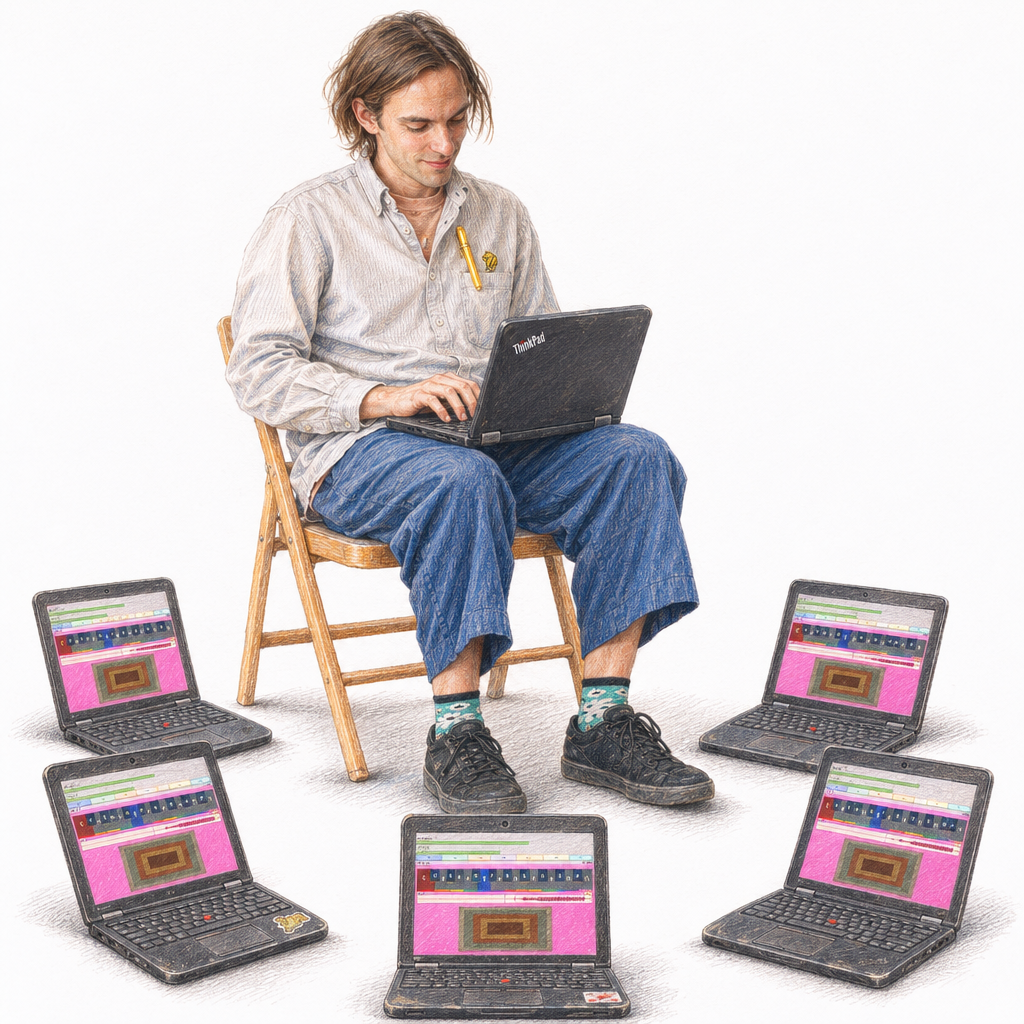
\includegraphics[width=0.44\textwidth]{figures/cover-nov}\par
\vspace{0.3em}
{\itshape\fontsize{14.5pt}{17pt}\selectfont\color{acpink} A Laptop Orchestra That Boots from a USB Stick}\par
\vspace{0.5em}
{\small\color{acgray} \handle{jeffrey} \,$\cdot$\, \ac{} \,$\cdot$\, ORCID \href{https://orcid.org/0009-0007-4460-4913}{0009-0007-4460-4913} \,$\cdot$\, November 20, 2026}\par
\vspace{0.55em}
{\color{acpink}\rule{\textwidth}{1.2pt}}
\vspace{0.5em}
\end{center}

\begin{quote}
\small\noindent\textbf{Abstract.}
A laptop orchestra can be made from laptops nobody wants. \acos{} boots a discarded PC from a USB stick straight into \np{}, an instrument whose keys play the notes they name: press \key{C}, hear C. There is no operating system to keep current. There is no software to install, no account, and no speaker array to build. On September 24, 2026, six salvaged laptops booted this way played a thirteen-minute spatial score in a ring around an audience in Los Angeles. A 774-second, 10,739-event score completed on all six. A musician who did not build the system, \handle{oskie}, then wrote a ten-lane groovebox for it on his own school-surplus ThinkPad.

The laptop orchestra began at Princeton in 2005 with stations of laptop, amplifier rack and hemispherical speaker. Since then more than 160 laptop ensembles have formed. Live coding took laptop music out of the conference and into the club. Free browser tools made a seat cost nothing on a current computer. This paper adds one more seat. It is for the computer that is no longer current and for the player who wants keys, not code. The paper describes the instrument. It gives the first ensemble measurements, the bad ones too. It names the tests that would show whether an orchestra of strangers' old laptops holds together.
\end{quote}
\vspace{0.5em}
}]

% ============ 1. INTRODUCTION ============

\section{Introduction}

The Princeton Laptop Orchestra began in 2005 as a proposition: that a laptop could be an orchestral instrument and a network of them an ensemble~\citep{trueman2006plork, trueman2007why}. Each station paired a laptop with a six-channel hemispherical speaker, an amplifier rack and controllers. The proposition held. PLOrk is still playing; it marked twenty years with a season that ended in a homecoming concert on April~2, 2026~\citep{kapilevich2025plork, princeton2026homecoming}.

To PLOrk something, in this paper, is to turn a computer into an instrument people sit down and play together. The question is who gets to. A PLOrk station needs an institution. A live coding set needs a current computer and a taste for typing code. Many people have neither. Many working laptops are on their way to a recycler.

\begin{figure*}[t]
\centering
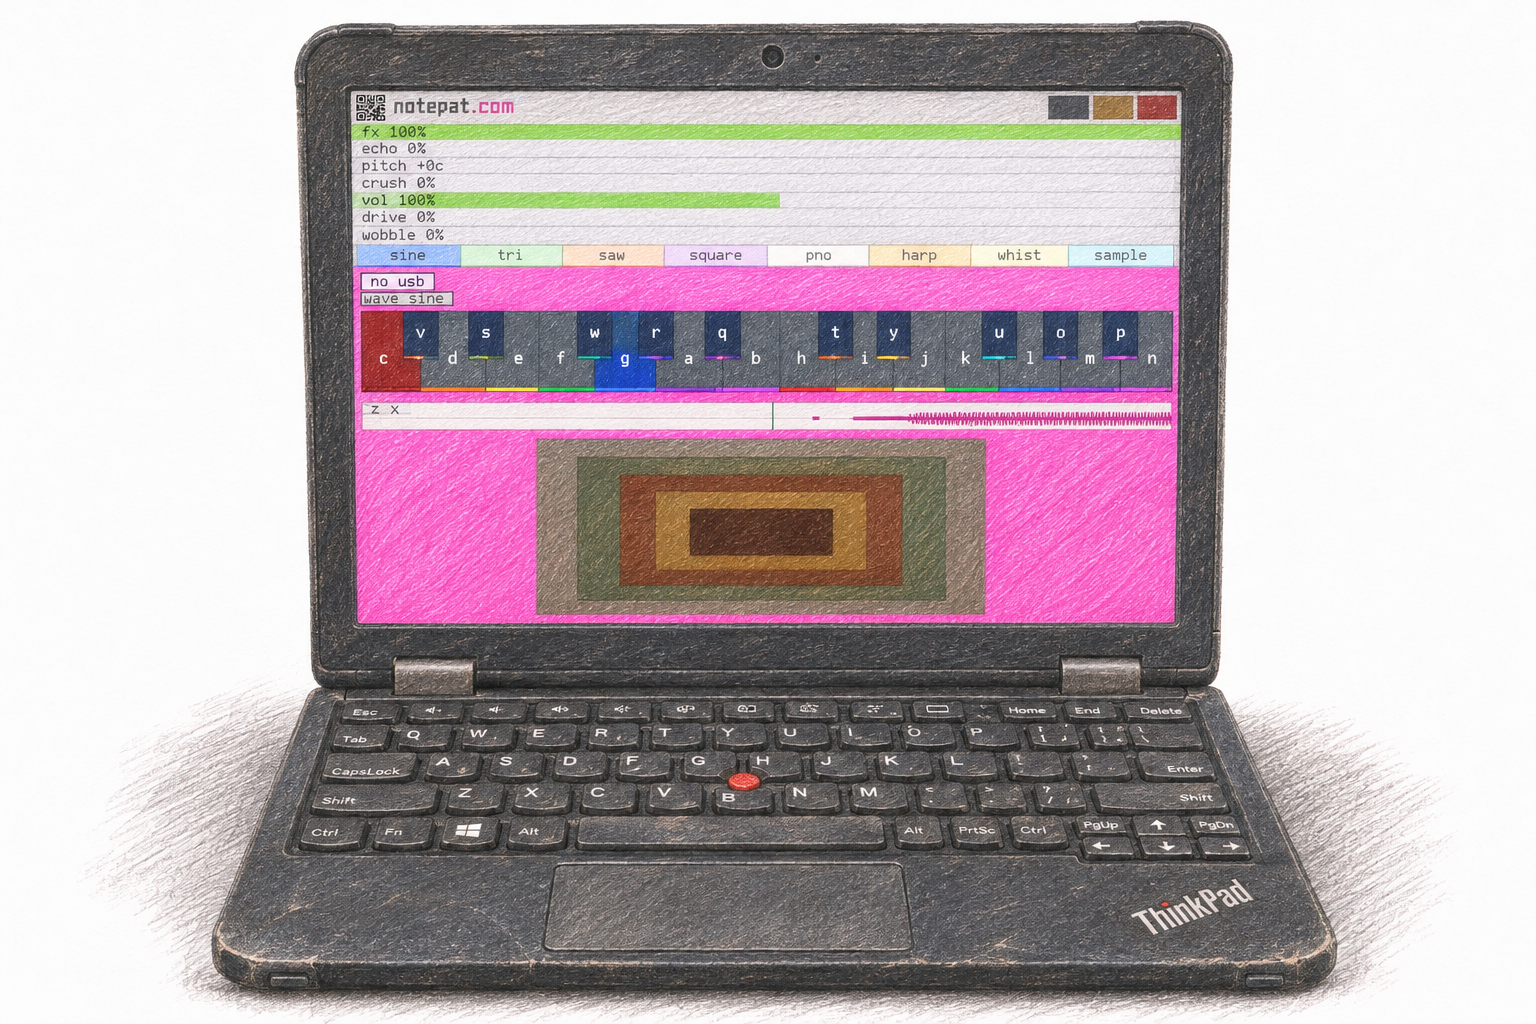
\includegraphics[width=0.66\textwidth]{notepat-laptop}
\caption{\textbf{\np{} on \acos{}.} A ThinkPad 11e running the instrument with \key{C} and \key{G} held, drawn in coloured pencil from a frame of the native piece's own source (\texttt{fedac/native/pieces/notepat.mjs}, commit \commit{ef70dc2b6a}) captured on November~20, 2026 at the machine's 1366$\times$768. The drawing is an illustration, not a photograph; its key letters, slider labels and tabs were checked against the captured frame. Each key on the strip carries the letter that plays it.}
\label{fig:notepat}
\end{figure*}

Take a laptop too old for its operating system. Put a USB stick in it. It boots into one program, a keyboard instrument whose keys are labelled with the notes they play. Put six of them in a room and they play one score. Hand one to a musician and he writes a new instrument for it.

All of that has happened once.

\begin{itemize}
  \item \textbf{The instrument.} \acos{} and \np{}, as built on November~20, 2026 (Section~\ref{sec:instrument}).
  \item \textbf{The ensemble.} Six laptops, one public performance, and the first measurements, good and bad (Section~\ref{sec:culturehub}).
  \item \textbf{A second author.} The first piece on the system by someone else (Section~\ref{sec:second}).
  \item \textbf{The lineage.} Laptop ensembles and live coding already left the university; what this adds to them (Sections~\ref{sec:landscape} and~\ref{sec:livecoding}).
  \item \textbf{The tests.} What would show the idea fails (Section~\ref{sec:tests}).
\end{itemize}

Seven machines is a chamber group. The planet is the direction. It is far.

% ============ 2. THE INSTRUMENT ============

\section{The Instrument}
\label{sec:instrument}

\acos{} boots a laptop into one program. There is no desktop and no browser. The first screen is \np{}, a chromatic keyboard instrument, and the first thing the machine can do is make a sound you chose~\citep{scudder2026os}. Figure~\ref{fig:notepat} shows it.

\subsection{The Keys}

The letters \key{C} \key{D} \key{E} \key{F} \key{G} \key{A} \key{B} play the notes they name, with sharps on \key{V} \key{S} \key{W} \key{R} \key{Q}. The upper octave runs \key{H} through \key{N}, with sharps on \key{T} \key{Y} \key{U} \key{O} \key{P}. One key shifts across nine octaves. A person who knows the names of the notes already knows where the first seven are.

The idea of a letter playing its own note is not mine. Children's Scratch pianos map the letter C to the note C, and a 2018 project plays a full chromatic octave that way~\citep{scudder2026laptop, scudder2026protocols}. What \np{} adds is the second octave and its use as a performance instrument. Fiebrink, Wang and Cook argued from inside PLOrk in 2007 that the laptop's own keys, trackpad and sensors were instruments in waiting~\citep{fiebrink2007laptop}. That is the lineage \np{} belongs to.

A keymap is a two-column table. It says which key plays which note. It is the part that travels: the same table runs in the browser, on \acos{} and in \href{https://prompt.ac/menuband}{Menu Band} on a Mac~\citep{scudder2026keymaps}. A plain-language version of that argument was edited by Casey Reas and published by UCLA's Social Software initiative~\citep{scudder2026keymapscore}. For an ensemble, a shared keymap does the work of a shared notation.

\subsection{The System}

On November~19, 2026 the published release was two files: a 15.1\,MB kernel and a 464.7\,MB initramfs. The C runtime is 36,957 lines in 29 files. A 598-line init script starts it and restarts it if it crashes. The image carries bash, git and an SSH daemon. People needed to write pieces on the machine. Pieces are JavaScript modules; 61 ship with the system.

The synthesizer has 96 voices and a 128-program General MIDI synth. Audio asks for 192\,kHz with a period of about a millisecond and gets it on some hardware. Measured key-to-sound latency is 3 to 4\,ms on HDA codecs and 12 to 22\,ms on the SOF audio most Chromebooks use~\citep{scudder2026latency}.

It boots machines with ordinary UEFI firmware. Since September~24, 2026 the same stick also boots a stock Intel Chromebook in developer mode, with no firmware change. The first was a Lenovo 500e. Nothing boots on ARM yet.

Updates are started by the person at the keyboard. In June I removed silent self-update. A machine should not reflash itself with nobody there. Now every machine needs someone to press the button.

% ============ 3. CULTUREHUB ============

\section{Six Laptops in a Room}
\label{sec:culturehub}

On September~24, 2026, at CultureHub in Los Angeles, six salvaged laptops running \acos{} played \emph{Note(s)pat(ial) Native}: eleven chapters, twelve minutes and fifty-four seconds. Five laptops stood in a pentagon around the audience and one was hand-held. A Windows PC under one seat served as subwoofer, five lights ran from two DMX outputs, and three Macs sang a second work through Menu Band. Figure~\ref{fig:ring} shows the layout and Figure~\ref{fig:score} the score.

\begin{figure}[t]
\centering
\begin{tikzpicture}[font=\footnotesize]
  % audience
  \node[circle, draw=acgray!70, dashed, line width=0.5pt, minimum size=2.5cm, text=acdark!80, align=center, font=\footnotesize] (aud) at (0,0.15) {audience};
  % seats
  \tikzset{seat/.style={draw=acdark, line width=0.5pt, fill=acpurple!10, rounded corners=1.5pt, inner sep=3.5pt, font=\footnotesize\ttfamily, minimum width=1.05cm}}
  \node[seat] (lf) at (-2.55, 1.75) {ac5};
  \node[seat] (rf) at ( 2.55, 1.75) {ac8};
  \node[seat] (rr) at ( 2.55,-1.55) {ac9};
  \node[seat] (lr) at (-2.55,-1.55) {ac4};
  \node[seat] (cr) at ( 0,   -2.25) {ac6};
  \node[seat, fill=acpink!14] (hd) at (0, 2.45) {ac0};
  \node[font=\footnotesize, text=acdark!80, anchor=south] at (hd.north) {in the performer's hands};
  \node[font=\footnotesize, text=acdark!80, anchor=south] at (lf.north) {left front};
  \node[font=\footnotesize, text=acdark!80, anchor=south] at (rf.north) {right front};
  \node[font=\footnotesize, text=acdark!80, anchor=north] at (lr.south) {left rear};
  \node[font=\footnotesize, text=acdark!80, anchor=north] at (rr.south) {right rear};
  \node[font=\footnotesize, text=acdark!80, anchor=north] at (cr.south) {centre rear};
  % conductor
  \node[draw=acgold, line width=0.6pt, fill=acgold!10, rounded corners=1.5pt, inner sep=3.5pt, font=\footnotesize] (con) at (0,-3.85) {conductor Mac: one downbeat, six clock offsets};
  \draw[acgold, thin, dashed] (con.north) -- ($(cr.south)+(0,-0.42)$);
\end{tikzpicture}
\caption{\textbf{The ring at CultureHub, September 24, 2026.} Six \acos{} laptops, five around the audience and one hand-held. A conductor Mac computed one downbeat, estimated each laptop's clock offset over the venue Wi-Fi, and every seat then played the shared score against its own audio clock.}
\label{fig:ring}
\end{figure}

\begin{figure}[t]
\centering
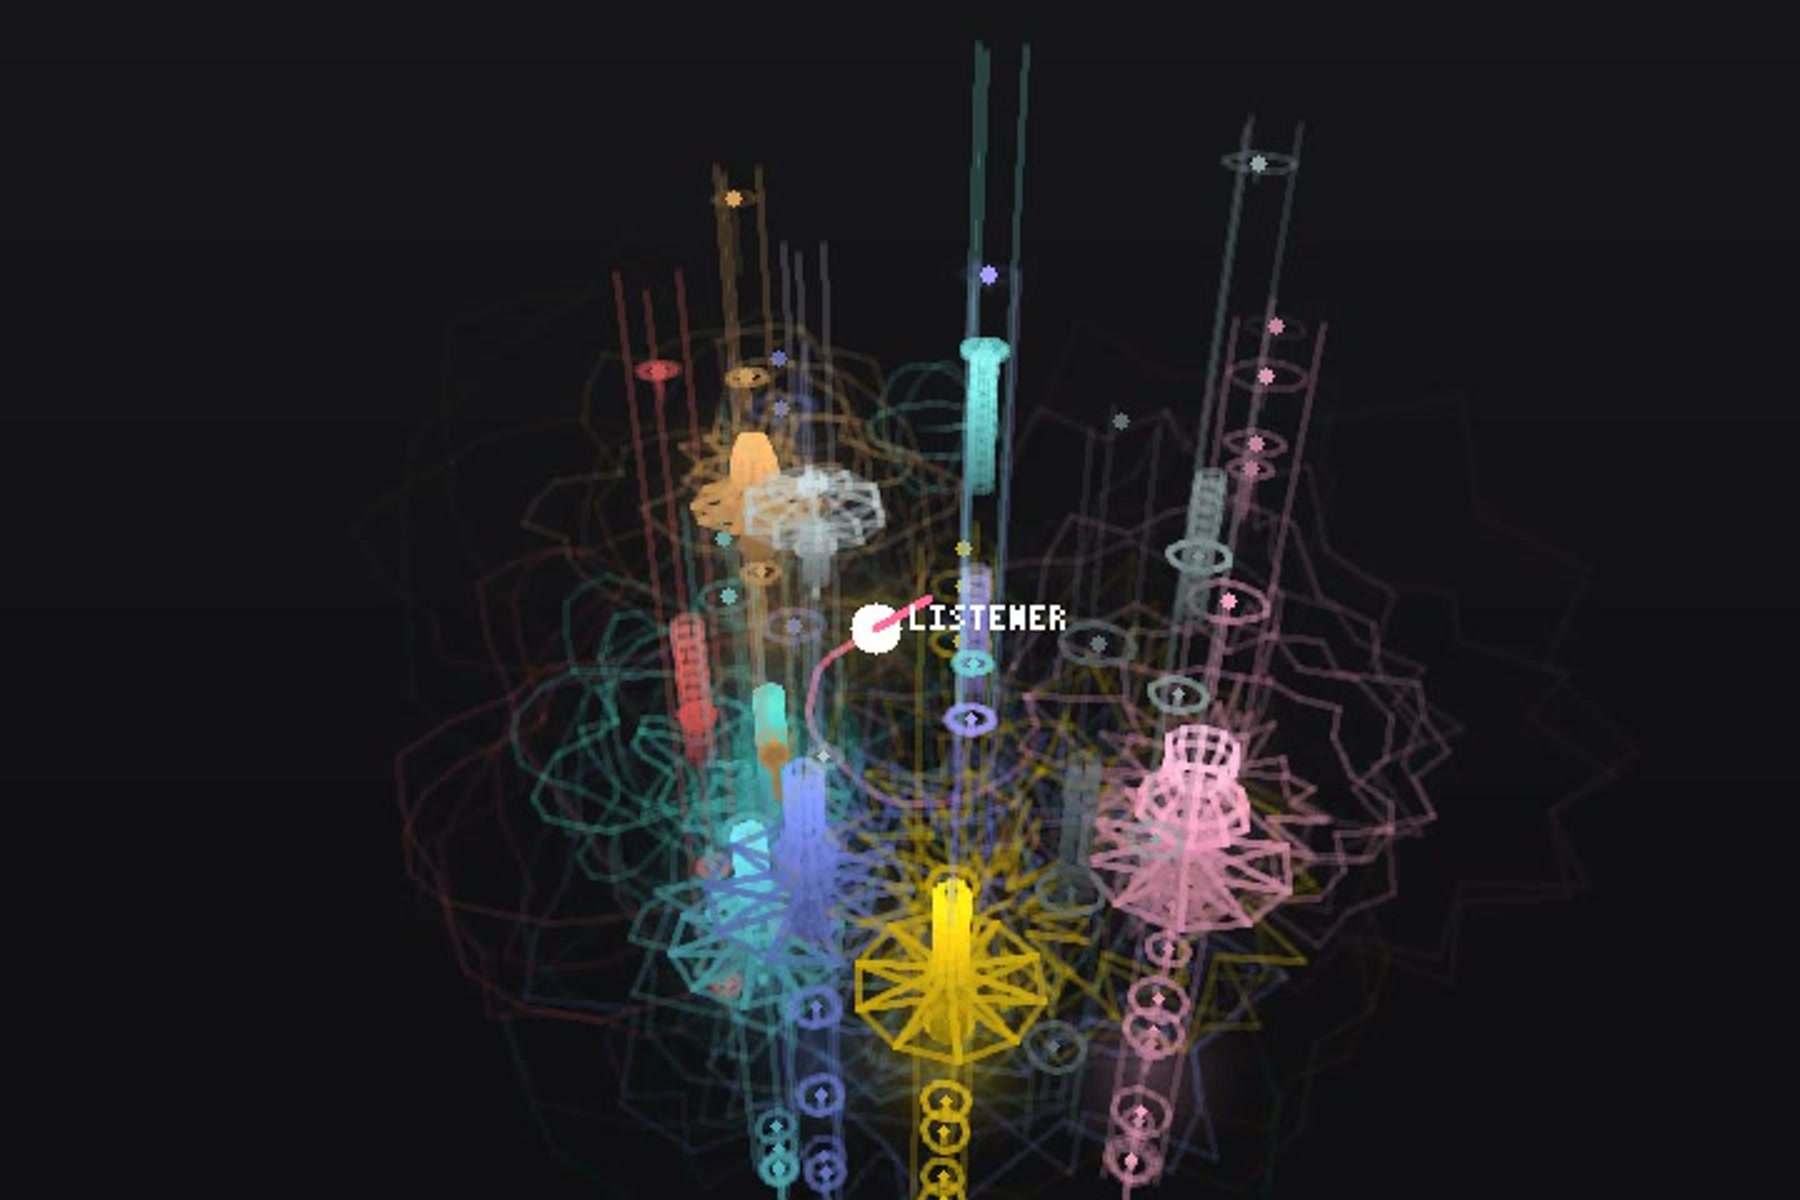
\includegraphics[width=\linewidth]{notespatial-score}
\caption{\textbf{The spatial score.} A view of the \emph{Note(s)pat(ial)} score: voices placed in space around a listener at the centre.}
\label{fig:score}
\end{figure}

\subsection{How It Was Synchronized}

Seat positions were assigned when the machines were set out. A conductor Mac computed one downbeat, probed each laptop's clock over HTTP fourteen times, and sent each seat a start time. Each laptop synthesized its part of the shared score against its own audio clock. For the show, all sounding layers were baked into per-seat stems.

Getting there took a list of addresses, tunnels from the conductor, and about a minute of preparation per piece. This was not six strangers forming an ensemble on a phone hotspot. It was one person who knew every machine.

\subsection{What Was Measured}

\begin{table}[t]
\centering
\begin{actable}{T{acsoftplum}|V{actablecream}}
  \acth{Measure} & \acth{Result} \\ \hline
  Stress score length & 774.4\,s \\ \hline
  Events, lanes & 10,739, 32 \\ \hline
  Laptops completing it & \held 6 of 6 \\ \hline
  Median frame rate per laptop & \held 52 to 58\,FPS \\ \hline
  Worst frame gap & \gone 4.28\,s \\ \hline
  Start lateness against audio clock & \held 2.76 to 14.23\,ms \\ \hline
  Stalls per seat during playback & \gone 130 to 380\,ms \\ \hline
  Clock probe round trip that aborted & \gone 46\,ms \\ \hline
  Sync as heard in the room & \partly not measured
\end{actable}
\caption{\textbf{CultureHub, September 24, 2026.} Teal marks a result that held, pink one that did not, gold one not yet measured. From the stress-run record and the fleet notes~\citep{scudder2026stress, scudder2026fleetdemo}.}
\label{tab:measured}
\end{table}

Table~\ref{tab:measured} is the first ensemble data this project has. All six laptops finished a thirteen-minute score with 128 instrument programs in play. Start times landed within about 14\,ms of each machine's audio clock.

The rest needs fixing. People assume local Wi-Fi is good to a few milliseconds. On the venue network, clock probes exceeded a 40\,ms limit and aborted. Every seat stalled for 130 to 380\,ms at some point during playback, and one laptop's worst gap between frames was 4.28 seconds. The scheduling fix that would hold timing through a stall sits on a branch that is not yet merged.

Nobody measured the sound in the room. I do not know how far apart the six laptops were as heard from a seat, and neither does anyone else.

\subsection{The Speakers}

The laptop's own speakers were meant to be the speakers. On the night there was also a subwoofer under one seat and the venue's surround system. Trueman's point stands. Laptop speakers carry a classroom. They did not carry that room.

% ============ 4. SECOND AUTHOR ============

\section{A Second Author}
\label{sec:second}

For most of its life one person, \handle{jeffrey}, wrote everything on this system. Of 1,088 commits to the OS between March~1 and November~20, 2026, one is by someone else. It is a groovebox.

On October~24 \handle{oskie} got a boot stick for his ThinkPad 11e and a one-page brief. The OS accepts a piece over the local network and reloads it while it runs. Over the next weeks he wrote \emph{Acid}~\citep{oskie2026acid}. It is a step groovebox. It has ten lanes, six grooves and a tempo range of 60 to 200\,BPM. Every sound is modelled on a Roland MC-909 and built from the engine's own voices. Until November~19 it lived only in his machine's memory. It vanished at each restart. That day it entered the tree, and the OS began keeping pushed pieces on the drive.

He also found a bug by ear. Hits were landing late about every three seconds. The cause was a display probe stalling the machine for roughly 120\,ms. A second musician heard what my tests had not.

Someone else changed the instrument. It is not only mine now.

% ============ 5. THE CENSUS ============

\section{Laptop Ensembles Were Never Only Academic}
\label{sec:landscape}

The laptop orchestra is not only a university form. Knotts and Collins surveyed 160 laptop ensembles in 2014~\citep{knotts2014politics}. They counted any group of three or more performers for whom the laptop is the main sound source. They did not call the list complete. A directory published in 2022 lists more than 160 ensembles active between 1995 and 2022 across the Americas, Europe, Asia, Australasia and Africa~\citep{woollard2022directory}. Princeton's own anniversary text says there are now hundreds~\citep{kapilevich2025plork}.

Knotts and Collins found that European groups were more often unaffiliated, with purely musical aims, and that university affiliation was far higher in North America. Groups with no institution predate PLOrk: the Mego Laptop Orchestra in 2000, Laptop Orchestra Tokyo in 2002, the Helsinki Computer Orchestra in 2003, Laptop Orchester Berlin in 2004. None of them followed what the survey calls the hierarchical ``PLOrkian model.''

Three cases matter most here.

\textbf{Sideband.} PLOrk's own professional spin-off formed in 2008 to take the model outside the yearly turnover of a class~\citep{princeton2026homecoming}.

\textbf{L2Ork.} Ivica Ico Bukvic built the Linux Laptop Orchestra at Virginia Tech to cut the cost. A seat was a netbook, a cheaper hemispherical speaker, a USB sound card and a Wiimote. It came to under \$800~\citep{bukvic2010l2ork}. By 2012 it had a satellite orchestra of fourth and fifth graders at the Boys \& Girls Club of Southwest Virginia~\citep{bukvic2012granular}. The 2010 paper names cost as ``the only formidable limitation'' on reaching schools.

\textbf{Medell\'{i}n.} In 2012, government-funded music schools for disadvantaged children in Medell\'{i}n contacted the authors of ChucK at Stanford. The children learned ChucK. In 2013 twenty of them, aged eight to thirteen, played the first algorave in Colombia~\citep{wilde2023livecoderas}. A children's laptop ensemble, outside any university, in the language PLOrk and SLOrk~\citep{wang2009slork} were written in.

What stayed on campus is the \emph{station model}: matched machines, hemispherical speakers, a director, a course. Laptop ensembles as a form went everywhere.

Cost is the usual explanation. L2Ork is the only orchestra I found that published a price per seat. It cut the price. It ran on free software. It aimed at schools. It stayed one university's project. A cheaper seat is needed. It is not enough.

% ============ 6. LIVE CODING ============

\section{Live Coding Already Left}
\label{sec:livecoding}

Live coding is where laptop ensemble music left the academy on purpose.

TOPLAP was founded on February~14, 2004 in Hamburg; its manifesto asks performers to ``show us your screens''~\citep{blackwell2022livecoding, toplap2024twenty}. The practice was already described in 2003~\citep{collins2003livecoding}. Alex McLean and Nick Collins coined ``algorave'' in 2011. McLean has said the name was partly a stand against how academic computer music conferences reacted to music with a beat~\citep{temkin2015mclean, nowthen2014algorave}. There is no licence and no permission: anyone may run one.

The International Conference on Live Coding has met nine times since Leeds in 2015, in Hamilton, Morelia, Madrid, Limerick, Valdivia, Utrecht, Shanghai and Barcelona; the tenth is in Antwerp in March 2027~\citep{iclc2027}. A 2025 paper counted 26 TOPLAP nodes as of September 2024 and none in Africa~\citep{anastasopoulou2025toplapathens}. The self-registered node page listed about 48 when I read it on November~20, 2026, including Cairo, Bengaluru, Yogyakarta, Bogot\'{a} and Mexico City~\citep{toplapnodes}. The two counts were made differently. I do not read the difference as growth. The week this paper was written, an algorave was on the programme of the Maebashi Biennale in Japan~\citep{tadokoro2026maebashi}.

\subsection{The Browser Is the Free Seat}

\acos{} needs no licence and no installation. The live coding community reached that years ago by another road. Strudel was written to make live coding more accessible by running entirely in the browser~\citep{roos2023strudel}. Estuary puts a whole networked ensemble in a shared browser session~\citep{ogborn2017estuary}. Sonic Pi, built for classrooms~\citep{aaron2016sonicpi}, has run in the browser since version 5.0.0 in August 2026~\citep{sonicpi2026web}. Table~\ref{tab:tools} sets them beside each other.

\begin{table}[t]
\centering
\begin{actable}{V{acsoftplum}|V{actablecream}|T{acsoftteal}}
  \acth{Tool} & \acth{Browser} & \acth{Needs} \\ \hline
  TidalCycles & \gone no & Haskell and SuperCollider \\ \hline
  Strudel & \held yes & a current browser \\ \hline
  Estuary & \held yes & a browser; an ensemble shares a session \\ \hline
  Sonic Pi & \held since 8/2026 & a browser, or the app \\ \hline
  Hydra, Gibber & \held yes & a browser \\ \hline
  \np{} on the web & \held yes & a browser \\ \hline
  \acos{} & \gone no & a USB stick and a laptop to boot it
\end{actable}
\caption{\textbf{What a seat requires.} Every tool here is free. The browser tools need a machine whose operating system and browser are still current; \acos{} needs a machine that can boot from USB.}
\label{tab:tools}
\end{table}

So a free seat already exists on any computer that runs a current browser. That leaves two openings.

The first is the machine whose browser is no longer current. A browser instrument depends on an operating system that still receives a browser. \acos{} does not.

The second is the interface. Live coding is typing code; the manifesto speaks of ``the glorification of the typing interface.'' \np{} is typing notes. A child who cannot read a pattern language can find the letter C.

\subsection{A Computer Is Not Access}

The same literature warns against treating hardware as access. Wilde and Duarte-Garc\'{i}a interviewed eleven Latin American live coders in 2022. Their interviewees reject the idea that a computer plus free software equals access, and one says plainly that not everyone has a computer to do this with~\citep{wilde2023livecoderas}. A decolonial critique in the same issue questions the Global North assumptions built into the tools~\citep{laramendoza2023unknowing}. A workshop for children in a regional Australian town in 2024 used only browser tools and still lost time to a tablet with no keyboard, headphones that would not pair, and a laptop that would not type one character~\citep{toplap2024kids}.

On the other side, a Karachi organiser describing Pakistan's first algorave in 2019 said he could pull out a laptop or a Raspberry Pi and start typing~\citep{wildcity2021algorave}. Cheap hardware matters to the people doing this. It is one of several scarce things, with teachers, rooms, time and networks.

% ============ 7. THE SURPLUS ============

\section{The Surplus}
\label{sec:surplus}

The raw material is old PCs. Canalys forecast in December 2023 that about 240 million of them, a fifth of the devices in use, would become e-waste because they could not run Windows~11~\citep{canalys2023windows10}. It was a forecast. It was not a count.

Support for Windows~10 ended on October~14, 2025. Microsoft then offered consumers extended security updates, and its page now says enrollment runs until the programme ends on October~12, 2027~\citep{microsoft2026esu}. I found no measured figure for machines scrapped or resold. The wave has not broken yet.

The Global E-waste Monitor reports 62 million tonnes of e-waste generated in 2022, 22.3\% documented as collected and recycled, and growth of 2.6 million tonnes a year~\citep{forti2024ewaste}. School Chromebook churn is documented separately~\citep{pirg2023chromebook}.

A surplus ThinkPad listed for about \$50 at refurbishers in March 2026. I did not re-survey prices, and I have no record of what the laptops in Section~\ref{sec:culturehub} cost. Treat it as an order of magnitude.

% ============ 8. SCALE ============

\section{From Six to a Planet}
\label{sec:scaling}

The scale so far:

\begin{itemize}
  \item \textbf{Seven} machines running \acos{} in one room, six playing and one showing lyrics.
  \item \textbf{Nine} machine names in the repository.
  \item \textbf{Two} people who have written a piece on the OS.
  \item \textbf{146} page loads of \np{} on the web in the thirty days to November~20, 2026: 48 on the main site and 98 on its own domain.
  \item \textbf{19,051} \href{https://kidlisp.com}{KidLisp} programs and \textbf{3,189} handles on the wider \ac{} network on the same day, which is the repertoire and the population the instrument sits inside.
\end{itemize}

That is a chamber group. Each new seat needs a person to boot it, a person to start its updates, and, on the evidence of September, a person to tune its network. Table~\ref{tab:future} lists what a larger ensemble needs and where each stands.

\begin{table}[t]
\centering
\begin{actable}{U{acsoftplum}{0.3\linewidth}|T{actablecream}}
  \acth{An ensemble needs} & \acth{State, November 2026} \\ \hline
  Composition tools & \held Shipped: a nine-track sequencer and sampler, a ten-lane groovebox, a turntable piece \\ \hline
  Spatial sound across laptops & \partly Shipped and performed; latency between seats uncalibrated \\ \hline
  ARM Chromebooks & \gone Not shipped. Intel Chromebooks boot on stock firmware \\ \hline
  Curriculum & \gone Not shipped. Printed score cards exist \\ \hline
  Mesh networking & \gone Not shipped
\end{actable}
\caption{\textbf{What a larger ensemble needs.} Teal is shipped, gold partial, pink not shipped.}
\label{tab:future}
\end{table}

The argument for scale is about the cost of one more seat. A browser seat costs nothing on a computer someone already has and that still gets a browser. An \acos{} seat costs a USB stick on a computer that can no longer be anything else. Neither removes the need for someone who knows how to run a room.

\subsection{Networks}

For ensembles in different places, latency is often called a compositional parameter. I have numbers from a neighbouring project. Two players in Los Angeles measured 193\,ms round trip through a relay in New Jersey. Through one in San Francisco they measured 64\,ms. Moving input to a datagram lane stopped a lost packet from holding up the ones behind it~\citep{scudder2026relay}. That work is for games. No music piece uses it yet. Native \np{} does send every note to a session server over UDP, which is a start.

% ============ 9. DEVICES AND PARTICIPATION ============

\section{Who Flashes the Stick}
\label{sec:devices}

\acos{} belongs with the devices that boot into one thing. The Nintendo Switch had sold 157.20 million units by September~30, 2026~\citep{nintendo2026units}, which shows that people will take a computer that does one thing at the press of a button.

The same pattern, fast boot into a single networked purpose on commodity hardware, describes autonomous military systems as well as it describes a child's first instrument. A dedicated device is a question of who decides what it boots. PLOrk's institution chose what its stations played. On a surplus laptop, the person holding the USB stick chooses. That is the centre of the argument.

Others reached the same politics by organizing differently. Knotts and Collins surveyed how laptop ensembles govern themselves and found directorless groups beside the hierarchical ones~\citep{knotts2014politics}. Ogborn's Cybernetic Orchestra was run as an open community of practice~\citep{ogborn2014scalable}.

Attali wrote that music runs ahead of political economy, and called the stage after mass recording \emph{composition}: everyone makes, and the line between performer and audience goes~\citep{attali1985noise}. Turino separates participatory music, judged by how many join in, from presentational music, judged by how it sounds to people sitting down~\citep{turino2008music}. Illich called a tool convivial when anyone can use it, without training, for ends they set themselves~\citep{illich1973tools}.

By those measures the September show was presentational: an audience sat inside a ring of laptops and listened to them play a score I wrote. The participatory moment so far is smaller. It is \handle{oskie}'s groovebox running on his own ThinkPad.

One Laptop per Child is the caution. Ames shows how a cheap machine with a custom operating system carried its makers' childhoods to children who had other needs, and how the charisma of the object stood in for teachers, repair and time~\citep{ames2019charisma}. A custom OS that boots into one program, built by one person and handed out with a brief, could repeat that story. Three things stand against it. The hardware already exists. An adult musician can use the instrument on the first day. I will measure before I hand machines out.

% ============ 10. TESTS ============

\section{Tests Registered, Not Yet Run}
\label{sec:tests}

On November~16 I wrote down six studies before collecting data, each with a result that would count as failure~\citep{scudder2026protocols}. One has run: a wider prior-art search, which showed that letter-named keys were not my invention. Five have not:

\begin{itemize}
  \item recall of the \np{} layout against the common DAW layout after 24 hours, 40 people per group;
  \item cold boot to first audible note, ten boots per laptop model, against an installed OS with a browser;
  \item latency and jitter with a solenoid tapper, 1,000 strikes per setup, then 24 human tappers;
  \item a listening test of liveness, 120 listeners;
  \item an audit of whether keystroke timing is used by a model, with a preset decision rule.
\end{itemize}

None of them is an ensemble study. This paper adds two. First, record the room: a microphone at the centre of the ring and one at each seat, and report the spread of onsets between laptops as heard. The pass line is a median spread under 20\,ms with no seat stalled. Second, hand six sticks to six people who have not used the OS, on a network I did not set up, and time how long until they are playing one score together. If that takes a conductor, tunnels and a list of addresses, the phrase ``anyone with an old laptop'' is not yet earned.

% ============ 11. LIMITATIONS ============

\section{Limitations}
\label{sec:limitations}

\textbf{One room, once.} All ensemble evidence comes from one evening. There is no audience count, no recording of the room, and no post-show report in the public record.

\textbf{No learners.} There is no user study, no classroom, no data on whether anyone learns anything. There is no curriculum.

\textbf{Boot time.} An early build booted in 7.3 seconds. The image has grown fivefold since and the boot time of a current build has not been measured.

\textbf{Hands on every machine.} Updates need a person at each laptop and a person to request each build.

\textbf{ARM.} The largest pool of surplus school hardware is ARM and nothing here boots on it.

\textbf{Speakers and keys.} Laptop speakers did not carry a venue. Laptop key matrices drop notes in chords of four or more, and stock keys carry no velocity~\citep{scudder2026laptop}.

\textbf{Nearly one author.} One outside commit in 1,088.

\textbf{Song mode.} The scrolling-lyric song mode that teaches a tune one note at a time exists in \np{} on the web. The native piece does not have it yet.

\textbf{Sources.} Some figures were read second-hand: the Canalys forecast through press coverage, and the 2022 directory through a tally I did not make by hand.

% ============ 12. CONCLUSION ============

\section{Conclusion}

In 2007 Dan Trueman asked ``Why a laptop orchestra?''~\citep{trueman2007why} and answered that networked computers could be a new kind of ensemble. He was right. So were the people in Tokyo, Helsinki and Berlin who were already doing it without a department. So were the twenty children in Medell\'{i}n. So is everyone who has typed a pattern into a browser at a club.

One seat was missing. It was the seat for the laptop nobody wants and the player who has never written code. That seat exists now. An old laptop boots from a stick into an instrument whose keys play the notes they name. Six of them have shared a score in front of an audience. A second person has written for it.

PLOrk'ing the planet is not a metaphor. It is seven machines, two authors, one room and a list of tests. Every one of the machines was salvaged. The planet is a long way from seven. The next seat costs a USB stick.

% ============ NOTE ON THE MARCH DRAFT ============

\section*{Note: Changes from the March 2026 Draft}

A working draft of this paper circulated in March 2026 marked not for citation. It made claims that the code, the September performance and the literature did not support. Table~\ref{tab:revised} lists each one beside what replaced it.

\begin{table*}[t]
\centering
\begin{actable}{U{acsoftplum}{0.2\textwidth}|T{acsoftpink}|T{acsoftteal}}
  \acth{Subject} & \acth{March 2026 draft} & \acth{This paper} \\ \hline
  Laptop ensembles & About thirty, all in universities & 160 surveyed in 2014; unaffiliated groups since 2000~\citep{knotts2014politics} \\ \hline
  Why they stayed & Cost per seat & Only L2Ork published a cost (under \$800); it cut cost and stayed on campus~\citep{bukvic2010l2ork} \\ \hline
  Free, no-install tools & Not discussed & Strudel, Estuary, Hydra, Gibber and, since August 2026, Sonic Pi run in a browser \\ \hline
  Surplus PCs & 240 million made obsolete & \partly A 2023 forecast; consumer patches now run to October 12, 2027~\citep{microsoft2026esu} \\ \hline
  Image size & 89\,MB, one file & 15.1\,MB kernel and 464.7\,MB initramfs \\ \hline
  Boot time & 7.3 seconds & \partly Not measured since March; a study is registered \\ \hline
  Runtime & 11,943 lines of C as PID~1, no shell & 36,957 lines; a child of a 598-line init script; bash, git and SSH on board \\ \hline
  Synthesizer & 32 voices & 96 voices and a 128-program General MIDI synth \\ \hline
  Updates & Automatic & Started by the person at the machine \\ \hline
  Ensemble & A diagram & Six laptops, one show, measured \\ \hline
  Authors of pieces on the OS & One & Two
\end{actable}
\caption{\textbf{The March draft against the evidence.} Pink column, the draft's claims. Teal column, what the repository, the release bucket and the literature showed on November~20, 2026. Gold marks a finding that is still partial or pending.}
\label{tab:revised}
\end{table*}

% ============ REFERENCES ============
\balance

{\footnotesize
\bibliographystyle{plainnat}
\bibliography{references}
}

% ============ COLOPHON ============

\vspace{1.2em}
\noindent\begin{minipage}{\linewidth}
\noindent{\color{acgray!60}\rule{\linewidth}{0.35pt}}\par\vspace{0.6em}
\noindent{\scriptsize\color{acgray}\raggedright
\textbf{Revision \paperrev} \,$\cdot$\, source \texttt{\paperhash} \,$\cdot$\, \url{https://papers.aesthetic.computer/plorking-the-planet-26-arxiv.pdf}\par
\smallskip
\textbf{Method.} Claims about \acos{} were checked on November~20, 2026 against the public repository, the release bucket and the live metrics endpoint; claims about laptop orchestras and live coding against the sources cited. \par
\smallskip
\textbf{Translations.} The Danish, Spanish, Japanese, Chinese and Russian editions still carry the March text.\par}
\end{minipage}

% Download box: the stick this paper is about.
\vspace{0.9em}
\noindent\begin{tikzpicture}
  \node[draw=acpink!80, line width=0.9pt, rounded corners=6pt, fill=acpink!5, inner sep=8pt] {%
    \begin{minipage}[c]{2.3cm}\centering
\includegraphics[width=2.3cm]{figures/qr-os}\end{minipage}%
    \hspace{8pt}%
    \begin{minipage}[c]{\dimexpr\linewidth-2.3cm-26pt\relax}\raggedright
    {\small\sffamily\bfseries\color{acpink!85!black} GET \MakeUppercase{\acos}}\par
    \vspace{0.3em}
    {\scriptsize\sffamily\color{acdark} Scan to download the image, write it to a USB stick, and boot an old laptop into \texttt{notepat}.\par
    \vspace{0.3em}
    \href{https://prompt.ac/os}{\texttt{prompt.ac/os}}\par}
    \end{minipage}%
  };
\end{tikzpicture}

\ifdefined\editionrev
\edef\acpaperrevnow{\paperrev}\edef\aceditionrevnow{\editionrev}%
\ifx\acpaperrevnow\aceditionrevnow
\vspace{0.9em}
\noindent\begin{tikzpicture}
  \node[draw=tezblue!80, line width=0.9pt, rounded corners=6pt, fill=tezblue!6, inner sep=8pt] {%
    \begin{minipage}[c]{1.1cm}\centering
\includegraphics[height=1.2cm]{figures/tez}\end{minipage}%
    \hspace{6pt}%
    \begin{minipage}[c]{\dimexpr\linewidth-1.1cm-24pt\relax}\raggedright
    {\small\sffamily\bfseries\color{tezblue!85!black} TEZOS EDITION OF \editionsize{} \,$\cdot$\, \#200tez}\par
    \vspace{0.3em}
    {\scriptsize\sffamily\color{acdark} Revision \paperrev{} of this paper was minted in \editiondate{} as an edition of \editionsize{} at \editionprice{} tez each. Every copy is this PDF.\par
    \vspace{0.3em}
    Collection: \emph{\editioncollection}\par
    Contract: \texttt{\editioncontract} \,$\cdot$\, token \texttt{\editiontoken}\par
    Minter: aesthetic.tez, \texttt{\editionminter}\par}
    \end{minipage}%
  };
\end{tikzpicture}
\fi
\fi

\end{document}
